%First stage



\begin{figure}[htbp]
    \centering
    
    \begin{subfigure}{\textwidth}
        \centering
        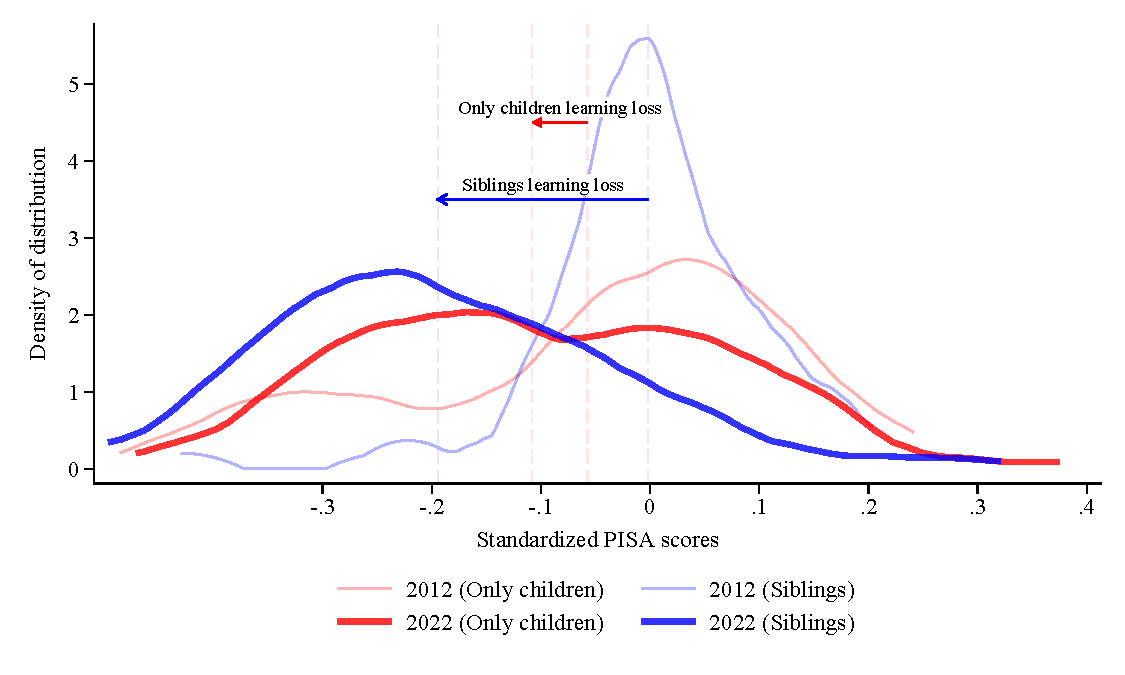
\includegraphics[width=\textwidth]{./FIGURES/Descriptive/PISA_distribution_2012_2022_PV4MATH.pdf}
        \caption{Learning gaps in Mathematics by year}
        \label{fig:1a}
    \end{subfigure}
    
    \vspace{1em} % Add some vertical space between subfigures
    
    \begin{subfigure}{\textwidth}
        \centering
        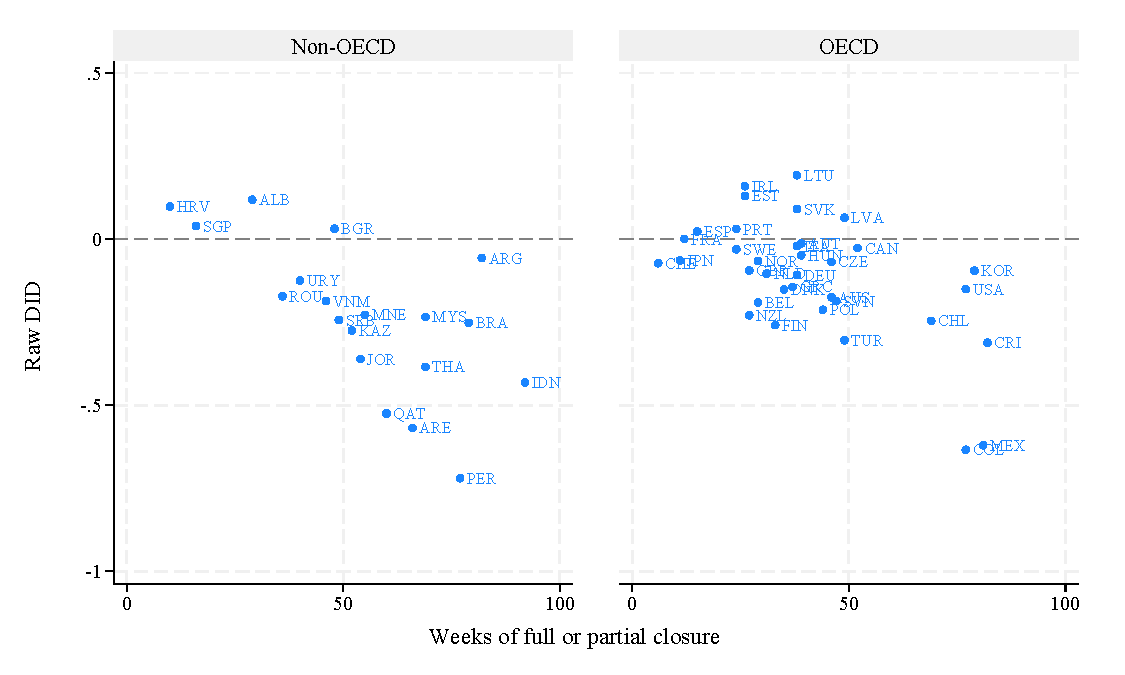
\includegraphics[width=\textwidth]{./FIGURES/Descriptive/PISA_raw_DID_PV4MATH_not_fully_open.pdf}
        \caption{Change in learning gaps by duration of school closure for OECD and Non-OECD countries.}
        \label{fig:1b}
    \end{subfigure}
    
    \caption{Learning gaps around the world}
    \label{fig:pisa}
\end{figure}


\begin{figure}[htbp]
    \centering
    
    \begin{subfigure}{\textwidth}
        \centering
        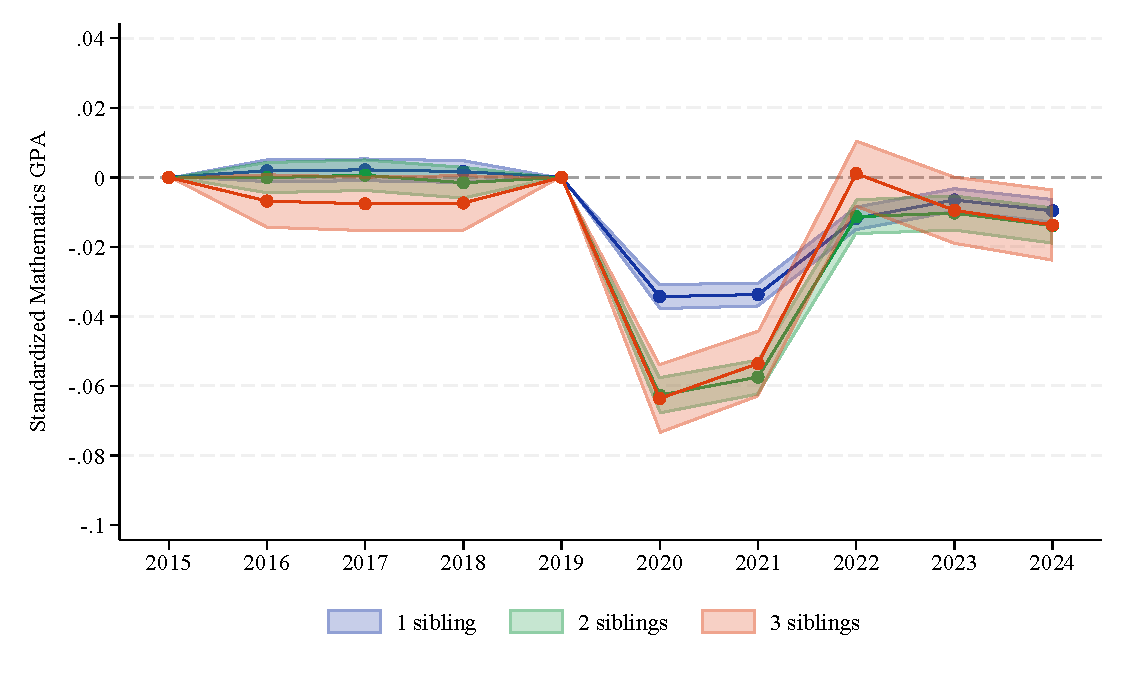
\includegraphics[width=\textwidth]{./FIGURES/Event Study/covid_event_bysibs_all_all_std_gpa_m_adj_Tsiblings_Soldest_4.pdf}
        \caption{Event Study}
        \label{fig:fig2a}
    \end{subfigure}
    
    \vspace{1em} % Add some vertical space between subfigures
    
    \begin{subfigure}{\textwidth}
        \centering
        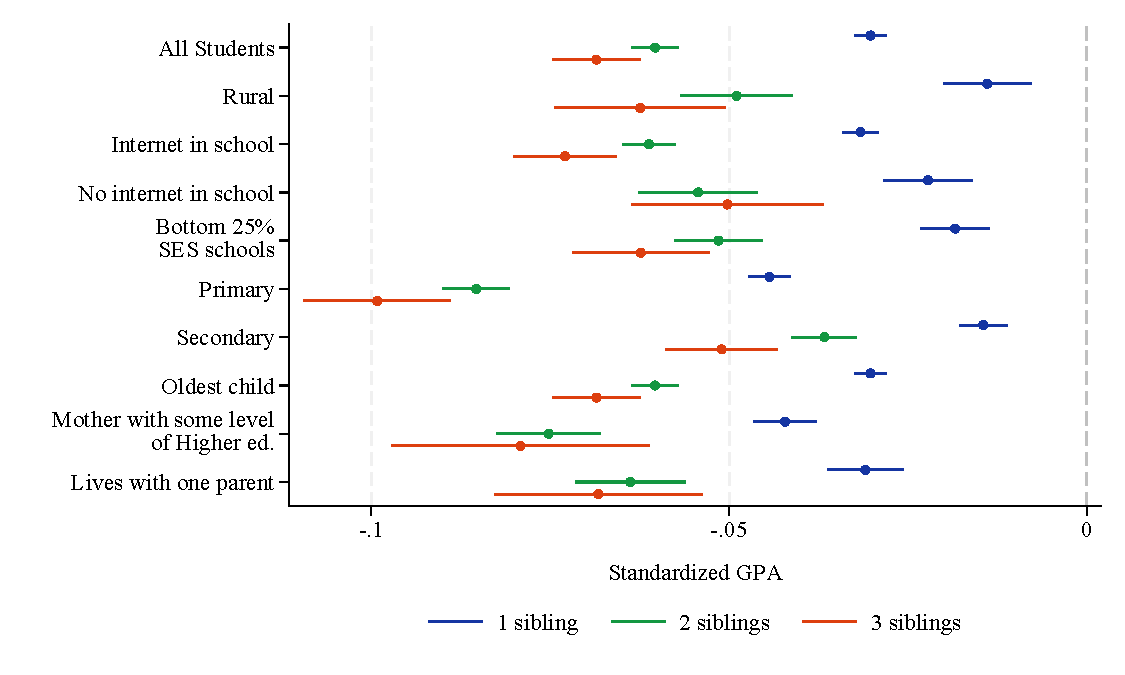
\includegraphics[width=\textwidth]{./FIGURES/TWFE/covid_twfe_summ_bysibs_all_20-21_gpa_m_adj_Tsiblings_Soldest_4.pdf}
        \caption{Change in gap between children with siblings and only childs}
        \label{fig:fig2b}
    \end{subfigure}
    
    \caption{Learning gap between only childs and siblings}
    \label{fig:fig2}
\end{figure}


\clearpage

%RD-first grade
\makeatletter
\@ifclassloaded{beamer}{%
       \centering
       \resizebox{0.6\textwidth}{!}%
}{%
       \begin{table}[!tbp]\centering\def\sym#1{\ifmmode^{#1}\else\(^{#1}\)\fi}
       \centering
       \caption{TWFE on 8th grade GPA and standardized exams controlling for baseline 2nd grade standardized exams}
       \label{tab:twfe_ece}
       \resizebox{0.95\textwidth}{!}%
}
{
\makeatother
\begin{tabular}{lcccc}
\toprule
\cmidrule(lr){2-5}
& \multicolumn{4}{c}{TWFE} \\
\cmidrule(lr){2-5}
& 1-3 siblings & 1 sibling & 2 siblings & 3 siblings  \\
\cmidrule(lr){2-2} \cmidrule(lr){3-3} \cmidrule(lr){4-4} \cmidrule(lr){5-5}
& (1) & (2) & (3) & (4) \\
\bottomrule
&  &  & &  \\
&  &  & &  \\
\multicolumn{5}{l}{Panel A: GPA } \\
Mathematics         &      -0.099***&      -0.011   &      -0.036***&      -0.059***\\
                    &     (0.009)   &     (0.009)   &     (0.011)   &     (0.015)   \\
                    &               &               &               &               \\
Observations        &     326,669   &     279,833   &     225,092   &     179,575   \\
 
&  &  & &  \\
Reading             &      -0.099***&      -0.010   &      -0.031***&      -0.034** \\
                    &     (0.009)   &     (0.009)   &     (0.010)   &     (0.015)   \\
                    &               &               &               &               \\
Observations        &     326,669   &     280,846   &     225,840   &     180,218   \\
 
&  &  & &  \\
\multicolumn{5}{l}{Panel B: Standardized Exams } \\
Mathematics         &      -0.034***&      -0.017** &      -0.044***&      -0.071***\\
                    &     (0.006)   &     (0.007)   &     (0.008)   &     (0.011)   \\
                    &               &               &               &               \\
Observations        &     409,527   &     282,640   &     227,403   &     181,370   \\
 
&  &  & &  \\
Reading             &      -0.013** &       0.002   &      -0.022***&      -0.046***\\
                    &     (0.006)   &     (0.006)   &     (0.008)   &     (0.011)   \\
                    &               &               &               &               \\
Observations        &     409,690   &     282,769   &     227,486   &     181,466   \\
 

\bottomrule
\end{tabular}
}
\@ifclassloaded{beamer}{%
}{%
       \end{table}
}

\makeatletter
\@ifclassloaded{beamer}{%
       \centering
       \resizebox{0.6\textwidth}{!}%
}{%
       \begin{table}[!tbp]\centering\def\sym#1{\ifmmode^{#1}\else\(^{#1}\)\fi}
       \centering
       \caption{TWFE on GPA by baseline resources}
       \label{tab:twfe_gpa_baseline_survey_1_pairall}
       \resizebox{0.65\textwidth}{!}%
}
{
\makeatother
\begin{tabular}{lccc}
\toprule
\cmidrule(lr){2-4}
& \multicolumn{3}{c}{TWFE} \\
\cmidrule(lr){2-4}
& 1 sibling & 2 siblings & 3 siblings  \\
\cmidrule(lr){2-2} \cmidrule(lr){3-3} \cmidrule(lr){4-4}
& (1) & (2) & (3)\\
\bottomrule
&  &  &  \\
&  &  &   \\
\multicolumn{4}{l}{\textit{Panel A: All studentes}} \\
\hspace{3mm}Mathematics&      -0.028***&      -0.061***&      -0.080***\\
                    &     (0.004)   &     (0.005)   &     (0.009)   \\
 
%&  &  &   \\
\hspace{3mm}Reading &      -0.018***&      -0.044***&      -0.052***\\
                    &     (0.004)   &     (0.005)   &     (0.009)   \\
                    &               &               &               \\
\hspace{3mm}Observations&   1,285,073   &   1,038,874   &     906,608   \\
 
&  &  &   \\
\multicolumn{4}{l}{\textit{Panel B: Low SES Households (Q1)}} \\
\hspace{3mm}Mathematics&      -0.009   &      -0.028***&      -0.061***\\
                    &     (0.007)   &     (0.009)   &     (0.014)   \\
 
%&  &  &   \\
\hspace{3mm}Reading &      -0.003   &      -0.016*  &      -0.040***\\
                    &     (0.007)   &     (0.009)   &     (0.014)   \\
                    &               &               &               \\
\hspace{3mm}Observations&     312,464   &     264,200   &     226,444   \\
 
&  &  &   \\
\multicolumn{4}{l}{\textit{Panel C: High SES Households (Q4)}} \\
\hspace{3mm}Mathematics&      -0.037***&      -0.065***&      -0.113***\\
                    &     (0.008)   &     (0.014)   &     (0.034)   \\
 
%&  &  &   \\
\hspace{3mm}Reading &      -0.029***&      -0.070***&      -0.017   \\
                    &     (0.008)   &     (0.014)   &     (0.034)   \\
                    &               &               &               \\
\hspace{3mm}Observations&     257,212   &     199,735   &     179,355   \\
 
&  &  &   \\
\multicolumn{4}{l}{\textit{Panel D: Households with no PC or Internet}} \\
\hspace{3mm}Mathematics&      -0.032***&      -0.079***&      -0.067***\\
                    &     (0.006)   &     (0.009)   &     (0.019)   \\
 
%&  &  &   \\
\hspace{3mm}Reading &      -0.023***&      -0.056***&      -0.051***\\
                    &     (0.006)   &     (0.009)   &     (0.019)   \\
                    &               &               &               \\
\hspace{3mm}Observations&     454,966   &     366,342   &     320,367   \\
 
&  &  &   \\
\multicolumn{4}{l}{\textit{Panel E: Households with both PC and Internet}} \\
\hspace{3mm}Mathematics&      -0.023***&      -0.035***&      -0.098***\\
                    &     (0.006)   &     (0.009)   &     (0.015)   \\
 
%&  &  &   \\
\hspace{3mm}Reading &      -0.008   &      -0.039***&      -0.061***\\
                    &     (0.006)   &     (0.009)   &     (0.015)   \\
                    &               &               &               \\
\hspace{3mm}Observations&     438,221   &     355,035   &     307,508   \\
 

\bottomrule
\end{tabular}
}
\@ifclassloaded{beamer}{%
}{%
       \end{table}
}

\makeatletter
\@ifclassloaded{beamer}{%
       \centering
       \resizebox{0.6\textwidth}{!}%
}{%
       \begin{table}[!tbp]\centering\def\sym#1{\ifmmode^{#1}\else\(^{#1}\)\fi}
       \centering
       \caption{WFE on GPA by baseline achievement and expectations}
       \label{tab:twfe_gpa_baseline_survey_2_pairall}
       \resizebox{0.65\textwidth}{!}%
}
{
\makeatother
\begin{tabular}{lccc}
\toprule
\cmidrule(lr){2-4}
& \multicolumn{3}{c}{TWFE} \\
\cmidrule(lr){2-4}
& 1 sibling & 2 siblings & 3 siblings  \\
\cmidrule(lr){2-2} \cmidrule(lr){3-3} \cmidrule(lr){4-4}
& (1) & (2) & (3)\\
\bottomrule
&  &  &  \\
&  &  &   \\
\multicolumn{4}{l}{\textit{Panel A: All studentes}} \\
\hspace{3mm}Mathematics&      -0.028***&      -0.061***&      -0.080***\\
                    &     (0.004)   &     (0.005)   &     (0.009)   \\
 
%&  &  &   \\
\hspace{3mm}Reading &      -0.018***&      -0.044***&      -0.052***\\
                    &     (0.004)   &     (0.005)   &     (0.009)   \\
                    &               &               &               \\
\hspace{3mm}Observations&   1,285,073   &   1,038,874   &     906,608   \\
 
&  &  &   \\
\multicolumn{4}{l}{\textit{Panel B: Student in bottom quartile of achievement}} \\
\hspace{3mm}Mathematics&       0.001   &      -0.042***&      -0.106***\\
                    &     (0.007)   &     (0.010)   &     (0.015)   \\
 
%&  &  &   \\
\hspace{3mm}Reading &       0.009   &      -0.036***&      -0.064***\\
                    &     (0.008)   &     (0.010)   &     (0.016)   \\
                    &               &               &               \\
\hspace{3mm}Observations&     261,349   &     220,666   &     193,655   \\
 
&  &  &   \\
\multicolumn{4}{l}{\textit{Panel C: Student in top quartile of achievement}} \\
\hspace{3mm}Mathematics&      -0.045***&      -0.101***&      -0.140***\\
                    &     (0.007)   &     (0.011)   &     (0.023)   \\
 
%&  &  &   \\
\hspace{3mm}Reading &      -0.032***&      -0.069***&      -0.090***\\
                    &     (0.007)   &     (0.011)   &     (0.023)   \\
                    &               &               &               \\
\hspace{3mm}Observations&     364,927   &     282,401   &     245,220   \\
 
&  &  &   \\
\multicolumn{4}{l}{\textit{Panel D: Max Expectation: Finish school}} \\
\hspace{3mm}Mathematics&      -0.003   &      -0.030   &      -0.054*  \\
                    &     (0.014)   &     (0.019)   &     (0.030)   \\
 
%&  &  &   \\
\hspace{3mm}Reading &      -0.027*  &      -0.031   &      -0.059*  \\
                    &     (0.015)   &     (0.019)   &     (0.031)   \\
                    &               &               &               \\
\hspace{3mm}Observations&      84,652   &      71,387   &      61,974   \\
 
&  &  &   \\
\multicolumn{4}{l}{\textit{Panel E: Max Expectation: 4-year college or grad school}} \\
\hspace{3mm}Mathematics&      -0.033***&      -0.067***&      -0.095***\\
                    &     (0.004)   &     (0.006)   &     (0.011)   \\
 
%&  &  &   \\
\hspace{3mm}Reading &      -0.022***&      -0.049***&      -0.073***\\
                    &     (0.004)   &     (0.006)   &     (0.011)   \\
                    &               &               &               \\
\hspace{3mm}Observations&   1,039,027   &     830,658   &     724,846   \\
 

\bottomrule
\end{tabular}
}
\@ifclassloaded{beamer}{%
}{%
       \end{table}
}



\clearpage
\makeatletter
\@ifclassloaded{beamer}{%
       \centering
       \resizebox{0.6\textwidth}{!}%
}{%
       \begin{table}[!tbp]\centering\def\sym#1{\ifmmode^{#1}\else\(^{#1}\)\fi}
       \centering
       \caption{Effects of younger sibling delaying school on older sibling standardized exams - 1 - m - a -  - 365}
       \label{tab:rd_summ_1_m_a_365}
       \resizebox{0.95\textwidth}{!}%
}
{
\makeatother
\resizebox{\textwidth}{!}{
\begin{tabular}{lccc}
\toprule
\cmidrule(lr){2-4}
& \multicolumn{3}{c}{Standardized GPA} \\
\cmidrule(lr){2-4}
& Pre-Covid & Covid & Post-Covid  \\
& 2018-2019 & 2020-2021 & 2022-2023  \\
\cmidrule(lr){2-2} \cmidrule(lr){3-3} \cmidrule(lr){4-4}
& (1) & (2) & (3)  \\
\bottomrule
&  &  &   \\
\multirow{2}{*}{\shortstack[l]{Younger sibling born after \\ school-entry cutoff}}&      -0.023***&      -0.001   &      -0.023***\\
                    &     (0.007)   &     (0.007)   &     (0.006)   \\
Local Linear        &         Yes   &         Yes   &         Yes   \\
                    &               &               &               \\
Observations        &     358,861   &     354,044   &     447,536   \\
Counterfactual mean &       0.058   &       0.020   &       0.050   \\
Bandwidth           &         365   &         365   &         365   \\
 

\bottomrule
\end{tabular}
}
\@ifclassloaded{beamer}{%
}{%
       \end{table}
}

\makeatletter
\@ifclassloaded{beamer}{%
       \centering
       \resizebox{0.6\textwidth}{!}%
}{%
       \begin{table}[!tbp]\centering\def\sym#1{\ifmmode^{#1}\else\(^{#1}\)\fi}
       \centering
       \caption{Effects of younger sibling delaying school on older sibling standardized exams and parental investment}
       \label{tab:rd_ece_index_365}
       \resizebox{0.95\textwidth}{!}%
}
{
\makeatother
\begin{tabular}{lccccc}
\toprule
& \multicolumn{2}{c}{Pre-Covid}  & \multicolumn{3}{c}{Post-Covid} \\
& \multicolumn{2}{c}{2018-2019}  & \multicolumn{3}{c}{2022-2024}  \\
\cmidrule(lr){2-3} \cmidrule(lr){4-6}
& Mathematics & Reading & Mathematics & Reading & Parental Investment  \\
& (1) & (2) & (3) & (4) & (5) \\
\bottomrule
&  &  &  & &  \\
\multirow{2}{*}{\shortstack[l]{Younger sibling born after \\ school-entry cutoff}}&      -0.025*  &      -0.023*  &      -0.009   &      -0.012   &      -0.035***\\
                    &     (0.014)   &     (0.012)   &     (0.013)   &     (0.010)   &     (0.013)   \\
Local Linear        &         Yes   &         Yes   &         Yes   &         Yes   &         Yes   \\
                    &               &               &               &               &               \\
Observations        &      86,605   &      86,602   &     104,983   &     105,064   &     101,766   \\
Counterfactual mean &      -0.105   &      -0.083   &       0.194   &       0.288   &      -0.004   \\
Bandwidth           &         365   &         365   &         365   &         365   &         365   \\
 

\bottomrule
\end{tabular}
}
\@ifclassloaded{beamer}{%
}{%
       \end{table}
}






